% fancytikzposter.tex, version 2.1
% Original template created by Elena Botoeva [botoeva@inf.unibz.it], June 2012
% 
% This file is distributed under the Creative Commons Attribution-NonCommercial 2.0
% Generic (CC BY-NC 2.0) license
% http://creativecommons.org/licenses/by-nc/2.0/ 


\documentclass{a0poster}

\usepackage{fancytikzposter} 
\usepackage[utf8]{inputenc}
\usepackage[spanish,mexico]{babel}


%%%%% --------- Change here if you want ---------- %%%%%
%% margin for the geometry package, must be changed before using the geometry package
%% default value is 4cm
% \setmargin{4}

%% the space between the blocks
%% default value is 2cm
% \setblockspacing{2}

%% the height of the title stripe in block nodes, decrease it to save space
%% default value is 3cm
% \setblocktitleheight{3}

%% the number of columns in the poster, possible values 2,3
%% default value is 2
% \setcolumnnumber{3}

%% the space between two or more groups of authors from different institutions
%% used in \maketitle
% \setinstituteshift{10}

%% which template to use
%% N1 simple, standard look, with a colored background and gray boxes
%% N2 board with nodes
%% N3 another standard look
%% N4 envelope-like look
%% N5 with a wave-like head, original idea taken from
%%%% http://fc09.deviantart.net/fs71/f/2010/322/1/1/scientific_poster_by_nabuy-d333ria.jpg
%\usetemplate{6}

%% components of the templates
%% (the maximal possible numbers are mentioned as the parameters)
% \usecolortemplate{4}
% \usebackgroundtemplate{5}
% \usetitletemplate{2}
% \useblocknodetemplate{5}
% \useplainblocktemplate{4}
% \useinnerblocktemplate{2}


%% the height of the head drawing on top 
%% applicable to templates N3, 4 and 5
% \setheaddrawingheight{14}


%% change the basic colors
%\definecolor{myblue}{HTML}{008888} 
%\setfirstcolor{myblue}% default 116699
%\setsecondcolor{gray!80!}% default CCCCCC
%\setthirdcolor{red!80!black}% default 991111

%% change the more specific colors
% \setbackgrounddarkcolor{colorone!70!black}
% \setbackgroundlightcolor{colorone!70!}
% \settitletextcolor{textcolor}
% \settitlefillcolor{white}
% \settitledrawcolor{colortwo}
% \setblocktextcolor{textcolor}
% \setblockfillcolor{white}
% \setblocktitletextcolor{colorone}
% \setblocktitlefillcolor{colortwo} %the color of the border
% \setplainblocktextcolor{textcolor}
% \setplainblockfillcolor{colorthree!40!}
% \setplainblocktitletextcolor{textcolor}
% \setplainblocktitlefillcolor{colorthree!60!}
% \setinnerblocktextcolor{textcolor}
% \setinnerblockfillcolor{white}
% \setinnerblocktitletextcolor{white}
% \setinnerblocktitlefillcolor{colorthree}




%%% size of the document and the margins
%% A0
% \usepackage[margin=\margin cm, paperwidth=118.9cm, paperheight=84.1cm]{geometry} 
\usepackage[margin=\margin cm, paperwidth=84.1cm, paperheight=118.9cm]{geometry}
%% B1
% \usepackage[margin=\margin cm, paperwidth=70cm, paperheight=100cm]{geometry}



%% changing the fonts
\usepackage{cmbright}
%\usepackage[default]{cantarell}
%\usepackage{avant}
%\usepackage[math]{iwona}
\usepackage[math]{kurier}
\usepackage[T1]{fontenc}


%% add your packages here
\usepackage{hyperref}
\usepackage{graphicx}




\title{OpenSCAD para diseño de modelos parametrizables en 2D y 3D}
\author{Pablo Vivar Colina\\
  LIDSOL, Facultad de Ingeniería, México
}


\begin{document}

%%%%% ---------- the background picture ---------- %%%%%
%% to change it modify the macro \BackgroundPicture
\ClearShipoutPicture
\AddToShipoutPicture{\BackgroundPicture}

\noindent % to have the picture right in the center
\begin{tikzpicture}
  \initializesizeandshifts
  % \setxshift{15}
  % \setyshift{2}


  %% the title block, #1 - shift, the default value is (0,0), #2 - width, #3 - scale
  %% the alias of the title block is `title', so we can refer to its boundaries later
  \ifthenelse{\equal{\template}{1}}{ 
    \titleblock{47}{1}
  }{
    \titleblock{47}{1.5}
  }

  %% a logo can be added to the title block
  %% #1 - anchor relative to the title block, #2 - shift, #3 - width, #3 - file name
  % \ifthenelse{\equal{\template}{2}}{ 
  %   \addlogo[south west]{(2,0)}{6cm}{unibz_b.png}
  % }{
  %   \addlogo[south west]{(2,0)}{6cm}{unibz_w.png}
  % }


  %% a block node, with the specified position (optional), title and the content
  %% #1 - where (optional), #2 - title, #3 - text
  %%%%%%%%%% ------------------------------------------ %%%%%%%%%%
  \blocknode{\Huge Plataforma}
  {
  
  \begin{center}
    \Huge OpenSCAD    
  \end{center}
  
  \begin{center}
  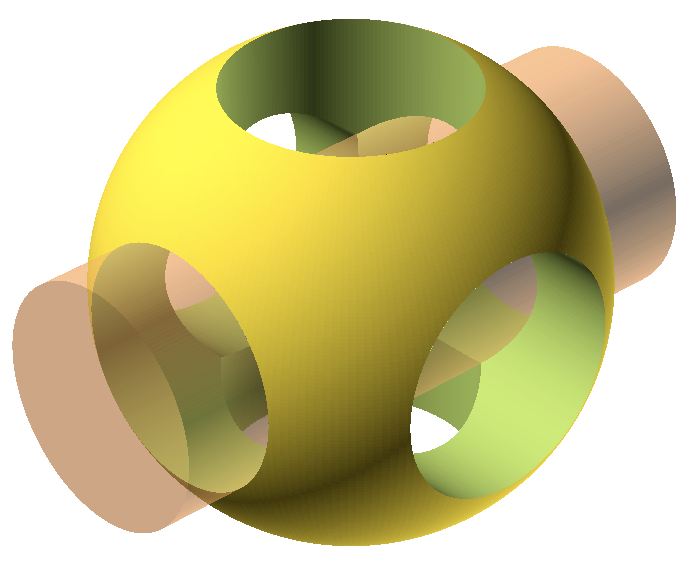
\includegraphics[scale=0.5]{OpenSCAD-logo.png}
  \end{center}
  
  \begin{center}
    \Large openscad.org/   
  \end{center}
  
  }
  

  
   \blocknode{\Huge Objetivo}{
  \Large
\begin{enumerate}
    \Large
 
    Hacer que los participantes del curso aprendan modelado parametrizable en 2D y 3D para la elaboración de planos que puedan ser manufacturados en máquinas de diseño (cortadora láser e impresora 3D).\\
\end{enumerate}
  }


  %% a callout block
  %% #1 - rotate angle (optional), #2 - from, #3 - where, #4 - width, #5 - text
  %%%%%%%%%% ------------------------------------------ %%%%%%%%%%
  
  
  %mensaje de texto de arduino
  %\calloutblock{($(box.center)+(-8,33)$)}
  %{($(box.center)+(5,31)$)}
  %{19cm}
  %{
  %\begin{center}
  %\includegraphics[scale=1.5]{illu-arduino-UNO.png}
  %\end{center}
  %}
  
 




  %% by default, the position of the new block node is right below the previous
  %% block node, stored in (currenty)
  %% box is the alias of the previous block, so we can refer to its boundaries

  %%%%%%%%%% ------------------------------------------ %%%%%%%%%%
  

 
  

  %%%%%%%%%% ------------------------------------------ %%%%%%%%%%
  
  
  %\blocknodew[($(currenty)-(3.5,0)$)]{30}{Variable Width Block Nodes} %
  
 
  
  \blocknode{\Huge Contacto} %
  { 
  
  \Large
  \begin{tabular}[t]{ll}
     
      \begin{minipage}{0.5\linewidth}
        \innerblock{\Large  Pablo Vivar Colina\\} {
       Correo:pablovc@tutanota.com\\
 
  Cel: 55-25-25-84-29 
        }
      \end{minipage}
      
    \end{tabular}
 
  }
  
  \blocknode{\Huge Notas y Recomendaciones}%
  {
    \Large
    El cupo es limitado a 10 integrantes, y es requisito llevar equipo propio.\\
  Para ingresar en el curso no es necesario tener conocimientos previos sobre programación o software, aunque es recomendado. \\
    

   %espacios en blanco
    %\vspace{5cm}
  }
  


  %%%%%%%%%% ------------------------------------------ %%%%%%%%%%
  %\plainblock[5]{($(currenty)+(4,2)$)}{17}{} %
  %{
    
   
   %¡Contáctanos si tienes dudas!\\

    %}
    
    
  %\getcurrentrow{note}

  %\plainblock{($(currentrow)-(xshift)+(yshift+3)$)}{32}{} 
  %{
  %\begin{center}
  %\includegraphics[scale=1]{arbol}
  %\end{center}
    
  %}
  
  


  %%%%%%%%%%%%% NEW COLUMN %%%%%%%%%%%%%%% 
  \startsecondcolumn 

  %%%%%%%%%% ------------------------------------------ %%%%%%%%%%


  
  %%%%%%%%%% ------------------------------------------ %%%%%%%%%%
  
  % ####Segunda columna
  
  \blocknode%
  {\Huge Temario}%
  {
  \Large 
  \begin{enumerate}
      \item Interfaz de código de Openscad
      \item Figuras 2D
      \item Comandos
      \item Figuras 3D
      \item Estructuras de iteración
      \item Módulos de pre-ensamblaje
            
      
  \end{enumerate}
  }


  
  %%%%%%%%%% ------------------------------------------ %%%%%%%%%%
  
  

 \blocknode{\Huge Lugar}%
  {
    \Large
  El curso se impartirá en El Laboratorio de Investigación y Software Libre, que se encuentra en el segundo piso del  edificio P en el Anexo de la Facultad de Ingeniería.
  \\
  Los días los cuales el curso se llevará a cabo serán del 29/01/18 al 02/02/18 de 11:00 a 14:00.
 
  \begin{center}
  
\includegraphics[scale=4]{LIDSOLlogoColor.png}
  \end{center}
  }
  
   \blocknode{\Huge Proyectos}%
  {
  \begin{center}
      
\includegraphics[scale=5]{DITANOVOA}
  \includegraphics[scale=0.65]{Idea161.jpg} 
  \end{center}
 
 \begin{center}
   
   \Large
   Consulta sobre El proyecto con piezas Ditac
    \href{http://www.facebook.com/DitacOficial}{\underline{aquí}}:\\
    facebook.com/DitacOficial
    
    y el proyecto de servicios 3D Idea 1.61 Ciencia, tecnología e ingeniería \href{http://www.facebook.com/idea161}{\underline{aquí}}:\\
    facebook.com/idea161
  
 \end{center}
   %espacios en blanco
    %\vspace{5cm}
  }
  
  %%%%%%%%%% ------------------------------------------ %%%%%%%%%%
  %\calloutblock{($(box.south east)-(8,-2)$)}
  %{($(box.south east)-(16,2)$)}
  %{30cm}
  %{
   % Para entrar en el curso sólo es necesario disponibilidad en el horario y ¡Muchas ganas de aprender!
  %}
  
  


  %% to place the next node centered vertically in the second column, we can
  %% obtain the y-coordinate of the previous node using macro
  %% \getcurrentrow{note}, where note is the alias of the callout node, and
  %% then specify the coordinate of the next node using coordinate (currentrow)
  %\getcurrentrow{note}


  %% a plain block
  %% #1 - rotate angle (optional), #2 - where, #3 - width, #4 - title, #5 - text
  %%%%%%%%%% ------------------------------------------ %%%%%%%%%%
  
  
  
  


   %%%%%%%%%%%%% NEW COLUMN %%%%%%%%%%%%%%% 
  %% (if column number is 3)
  \startthirdcolumn

  %%%%%%%%%% ------------------------------------------ %%%%%%%%%%
  

    
    
  }



\end{tikzpicture}


\end{document}

